\documentclass[tikz,border=7pt]{standalone}
% end preamble
\usepackage[e]{esvect}
\usetikzlibrary{calc, angles}
\tikzset{
  line/.style = {
    shorten <=-3mm, shorten >=-3mm
  },
  vector/.style = {
    thick,-latex
  },
  dot/.style = {
    insert path={
      node[scale=2]{.}
    }
  },
  perp/.style = {
    draw,
    angle eccentricity=.5,
    angle radius=2mm,
    pic text=.
  }
}
\begin{document}
  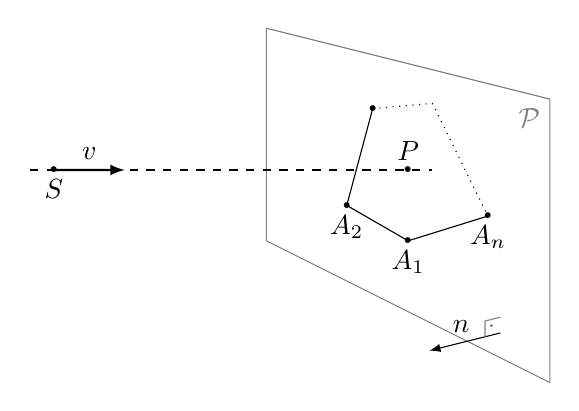
\begin{tikzpicture}[scale=0.9]
    % le plan
    \draw[gray]
      (0,0) coordinate (P1)
      -- ++(0,3) coordinate (P2)
      -- ++(4,-1) coordinate (P3)
      -- ++(0,-4) coordinate (P4)
      -- cycle
      (P3) node[below left]{$\mathcal{P}$}
    ;
    % les points A1,...
    \path
      (2,1)
      +(-90:1)   coordinate (A1)
      +(-150:1)  coordinate (A2)
      +(120:1)   coordinate (A3)
      +(70:1)    coordinate (A4)
      +(-30:1.3) coordinate (A5)
    ;
    % le vecteur normal
    \path (P4)
      ++(-.7,.7) coordinate (N)
      +(-1,-.25) coordinate (Na)
      +(0,1) coordinate (Nn)
      (N) edge[-latex] node[above, pos=.55]{$\vv{n}$} (Na)
      pic[perp,gray]{right angle=Nn--N--Na}
    ;
    % le polygone
    \draw (A5) -- (A1) -- (A2) -- (A3) ;
    \draw[dotted] (A3) -- (A4) -- (A5) ;
    % le rayon
    \path
      (-3,1) coordinate (S)
      (2,1) coordinate (P)
      ($(S)!1cm!(P)$) coordinate (v)
    ;
    \draw
      (S) edge[line, dashed] (P)
    ;
    \draw
      (S) edge[vector] node[above, sloped]{$\vv{v}$} (v)
    ;
    % les points
    \path
      (S) [dot] node[below]{$S$}
      (P) [dot] node[above]{$P$}
      (A1) [dot] node[below]{$A_1$}
      (A2) [dot] node[below]{$A_2$}
      (A3) [dot]
      (A5) [dot] node[below]{$A_n$}
    ;
  \end{tikzpicture}
\end{document}
